\chapter{Development}
\section{Considerations}
\subsection{Xcorr}
\subsubsection{Theory}
Cross-correlation is a method used for comparing two signals. This can for example be with the purpose of finding specific features, patterns or identical signals.


\begin{equation}
\label{eq:xcross}
\centering
(f\star g)(t)=\sum\limits_{m=-\infty}^{m=\infty}f(t)*g(t+m)
\end{equation}
The equation in \ref{eq:xcross} is the mathematical expression of cross-correlation of discrete functions.

In figure \ref{fig:xcrossSample} two signals are present. We can use cross-correlation to find out how much these two signals are similar. This can be done using equation \ref{eq:xcross}. Since our signal doesn't go to $\infty$, but only to 7, we will let $m=-7$ to $m=7$, so our equation will be the one shown in \ref{eq:xcross2}.

\begin{equation}
\label{eq:xcross2}
\centering
(f\star g)(t)=\sum\limits_{m=-7}^{m=7}f(t)*g(t+m)
\end{equation}

We can establish from the graph that the two signals have consist of the two following data sets:
Green: \[0,1,2,1,0,0,0\]
Blue: \[0,0,0,1,2,1,0\]
These are the data points from 1-7. Any data point outside of that range will be zero. We will also use $t=-7$ to $t=7$ to cover the negative side in case of a left side shift.

We can then, following equation \ref{eq:xcross2}, calculate the cross-correlation:

\begin{center}
$(f\star g)(-7)=f(-7)*g(-7+(-7)+f(-7)*g(1+(-6))+...+f(-7)*g(-7+6)+f(1)*g(-7+7)$\\
$(f\star g)(-6)=f(-6)*g(-6+(-7)+f(-6)*g(2+(-6))+...+f(-6)*g(-6+6)+f(2)*g(-6+7)$\\
$(f\star g)(-5)=f(-5)*g(-5+(-7)+f(-5)*g(3+(-6))+...+f(-5)*g(-5+6)+f(3)*g(-5+7)$\\
$(f\star g)(-4)=f(-4)*g(-4+(-7)+f(-4)*g(4+(-6))+...+f(-4)*g(-4+6)+f(4)*g(-4+7)$\\
$(f\star g)(-3)=f(-3)*g(-3+(-7)+f(-3)*g(5+(-6))+...+f(-3)*g(-3+6)+f(5)*g(-3+7)$\\
$(f\star g)(-2)=f(-2)*g(-2+(-7)+f(-2)*g(6+(-6))+...+f(-2)*g(-2+6)+f(6)*g(-2+7)$\\
$(f\star g)(-1)=f(-1)*g(-1+(-7)+f(-1)*g(7+(-6))+...+f(-1)*g(-1+6)+f(7)*g(-1+7)$\\
$(f\star g)(0)=f(0)*g(0+(-7)+f(0)*g(0+(-6))+...+f(0)*g(0+6)+f(0)*g(0+7)$\\
$(f\star g)(1)=f(1)*g(1+(-7)+f(1)*g(1+(-6))+...+f(1)*g(1+6)+f(1)*g(1+7)$\\
$(f\star g)(2)=f(2)*g(2+(-7)+f(2)*g(2+(-6))+...+f(2)*g(2+6)+f(2)*g(2+7)$\\
$(f\star g)(3)=f(3)*g(3+(-7)+f(3)*g(3+(-6))+...+f(3)*g(3+6)+f(3)*g(3+7)$\\
$(f\star g)(4)=f(4)*g(4+(-7)+f(4)*g(4+(-6))+...+f(4)*g(4+6)+f(4)*g(4+7)$\\
$(f\star g)(5)=f(5)*g(5+(-7)+f(5)*g(5+(-6))+...+f(5)*g(1+6)+f(5)*g(5+7)$\\
$(f\star g)(6)=f(6)*g(6+(-7)+f(6)*g(6+(-6))+...+f(6)*g(2+6)+f(6)*g(6+7)$\\
$(f\star g)(7)=f(7)*g(7+(-7)+f(7)*g(7+(-6))+...+f(7)*g(3+6)+f(7)*g(7+7)$\\
\ \\
$(f\star g)(1)=$\\
$(f\star g)(2)=$\\
$(f\star g)(3)=$\\
$(f\star g)(4)=$\\
$(f\star g)(5)=$\\
$(f\star g)(6)=$\\
$(f\star g)(7)=$\\
\end{center}

Instead of letting m be in the range of $-\infty$ to $\infty$, we will let our sample size control the range, as in equation \ref{eq:xcrossN}
\begin{equation}
\label{eq:xcrossN}
\centering
(f\star g)(t)=\sum\limits_{m=-N}^{m=N}f(t)*g(t+m)
\end{equation}


\subsubsection{Test Matlab}
Before we went any further with the project we investigated which kind of signals which was good to send. We did that by generating a signal, made a delay and then cross-correlated these two signals, chirp, sinusoid and noise.
We tried three different signals\\
\textbf{Chirp}:\\
We started with a chirp. We did that because of gut feeling. We thought this would be the best signal to send mostly because it was controlled and not random, and the signal changed characteristic over time.\\
Below is shown the code we used to generate the signal, make the delay and do the cross-correlation:
\begin{lstlisting}[language=Matlab,frame=lrtb,label=Matlab Code for Chirp Cross-correlation]
Fs=48000;                                       % Sample frequency
t = [0:1/Fs:1];                                % Timeinterval and length
Frq1=14000;                                     % Start frequency for chirp
Frq2=14100;                                     % End frequency for chirp
delay = 2000;                                   % Signal Delay
Chirp_signal=chirp(t,Frq1,1,Frq2);              % Chirp signal generation
Chirp_delayed=[zeros(1,delay) Chirp_signal];    % Chip delay generation
Chirp_xcorr=xcorr(Chirp_signal,Chirp_delayed);  % Cross-correlation
LengthChirp_xcorr=length(Chirp_xcorr)           % Calculate length of Xcorr
[XmaxChirp_xcorr,YmaxChirp_xcorr]=max(Chirp_xcorr) % Find maximum value
Delay_calcX1X2=((LengthChirp_xcorr+1)/2)-YmaxChirp_xcorr % Calculate Delay
\end{lstlisting}
Below is the plot of the cross-correlation. It shows clearly where the to signal overlap.\\
\begin{figure}[H]
\centering
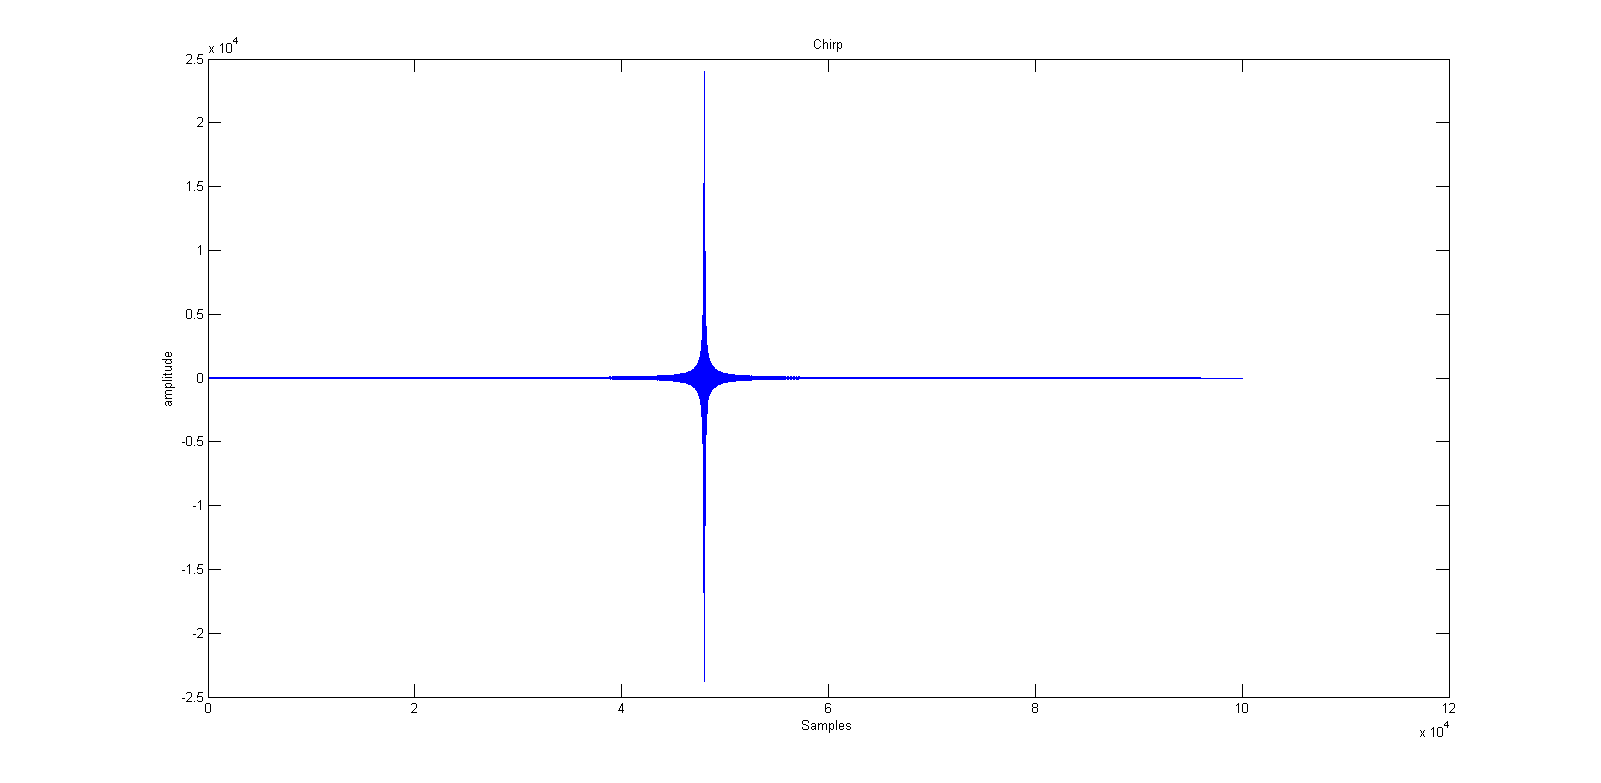
\includegraphics[width=0.6\textwidth]{billeder/chirp_xcorr_fig}
\caption{Plot of Cross-correlation of chirp signals}
\label{fig:chirp_xcorr_plot}
\end{figure}
The figure clearly shows where the two signals perfectly overlap. So the chirp seems like a good signal to use. although it isn't perfectly sharp in one sample it is quite distinct.\\
\textbf{Sinusoid}:\\
Similar code as the chirp was used to make two sinusoid signal. Below is a plot of a 14kHz sinus delayed with the same amount as the chrip signal.\\
\begin{figure}[H]
\centering
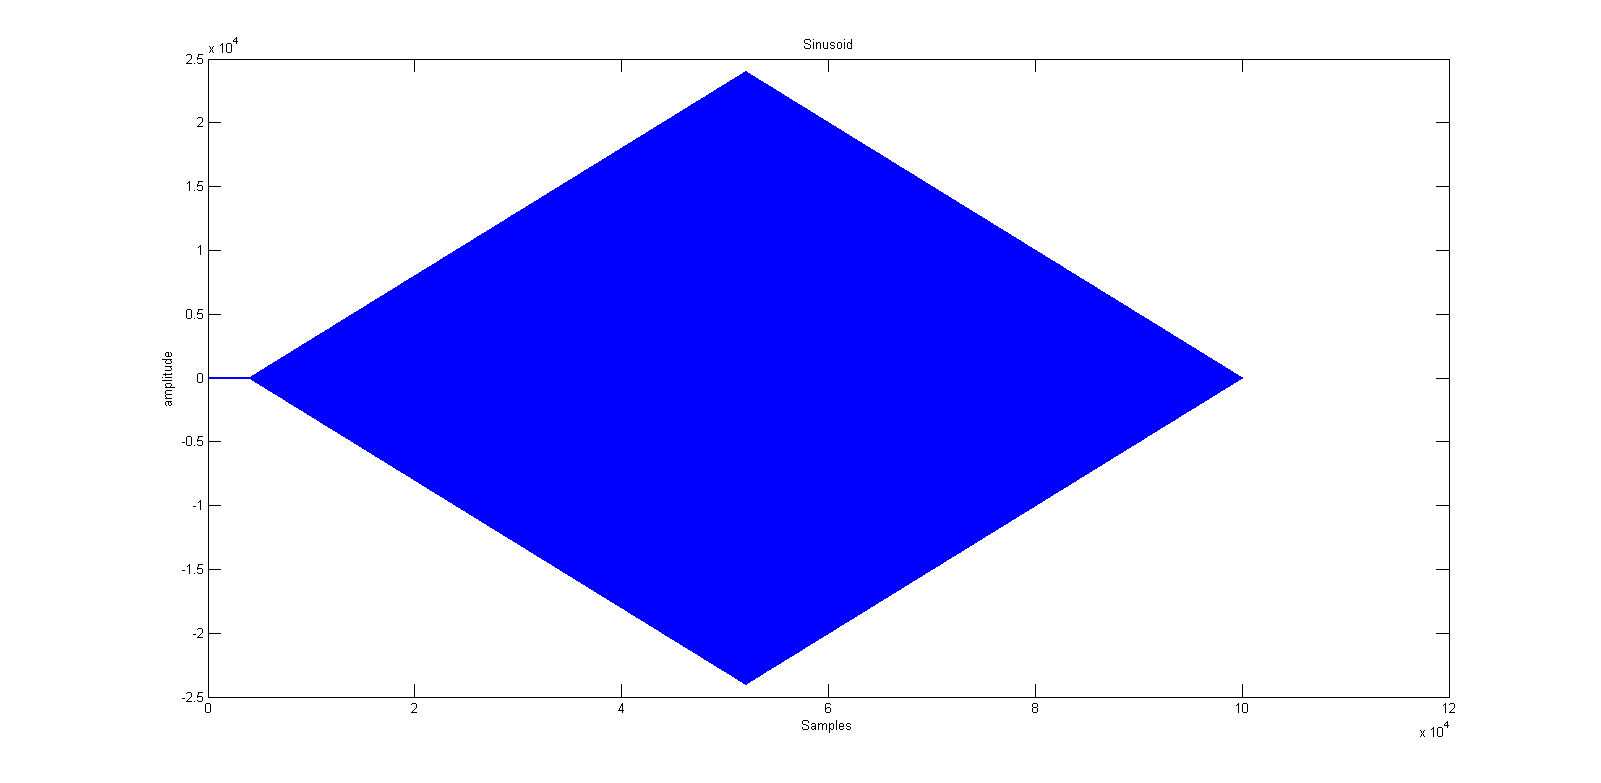
\includegraphics[width=0.6\textwidth]{billeder/sinus_xcorr_fig}
\caption{Plot of Cross-correlation of sinusoid signal}
\label{fig:sinus_xcorr_plot}
\end{figure}
This cross-correlation doesnt have as nice a peak as the chirp did and therefore we discarded using a sinusoid. The correlation looks like this because the sinus will make a spike every period because the periods will overlay eachother, this will increase until the signals completely overlays eachother.\\
\textbf{Noise}:\\
Lastly we tried generating a noise signal using the built-in function wgn (white gaussian noise). Below is shown the cross-correlation of the noise signals.\\
\begin{figure}[H]
\centering
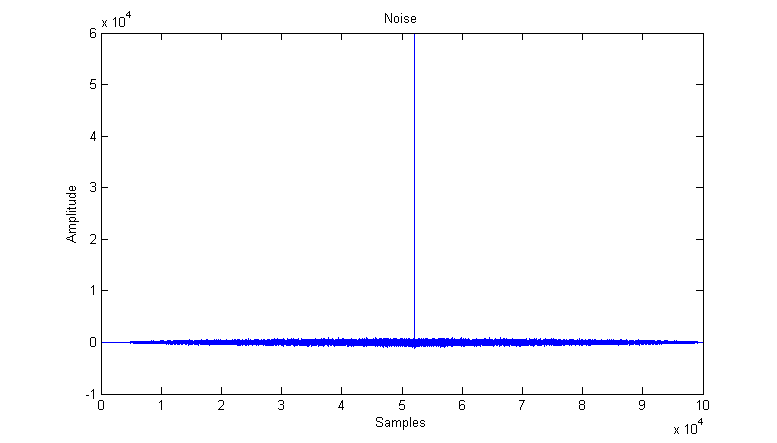
\includegraphics[width=0.6\textwidth]{billeder/noise_xcorr_fig}
\caption{Plot of cross-correlation of noise signal}
\label{fig:noise_xcorr_plot}
\end{figure}
This correlation made an even harder spike then the chirp. This is because of the fact that the  two noise signal only are similar in a very specific point. When they are not completely overlaying each other most samples end up cancelling each others.
\subsection{Findings based on examination in matlab}
It is clear that the chirp as well as the noise are very distinct peaks where the signals overlap. 
\subsection{Output}
\textbf{UART}:\\
VisualDSP++ comes with an example project for UART. We tried running the example project but we had no luck. We could not get the example project to work. We searched the internet for other example projects but still, we could not get them to work. \\
\textbf{Sound}:\\
The original scope of our project was to have an audio source as our output, while using a sound to measure distance. This worked well since we already had the knowledge from the talkthrough on how to output sound.\\
We have a multitude of ways to create the sound we are playing. We could either create a sound in matlab and load it or we could create it directly on the blackfin. For testing purposes we chose the matlab solution. This would mean that once we have made the soundbits we wanted to use, we would have to convert them to a format known by the blackfin.
\section{Convert to BF}
The blackfin has a small "hack" when it comes to loading sound from memory:
\begin{lstlisting}[language=C]
short sound_buffer[length_of_signal] = { 
#include "signal_you_want_to_use.hex"
};
\end{lstlisting}
This means we have to convert our sound array to a hex format. The first thing we do when converting is reducing the amplitude of the signal to make sure it fits in a "c style short" datatype. Then we use a function "mydec2hex" which is an improved version of matlabs built-in function "dec2hex". After converting to hex-format we use the file descriptor to save the data into a hex file. The hex file is put in the project folder in VisualDSP++ and the codehack is put where you initialize your variables.

\section{Blackfin}
\textbf{Memory}:\\
The blackfin has 2 types of memory: Internal and external. The internal SRAM consist of fast memory that is close to the processor.  As previously mentioned the L1 Data SRAM size is 32K Bytes. If we were to chose large arrays for our sound array we could enable the external SDRAM as well. This would provide us with a grand total of 132M bytes of memory. The SRAM is based on Harvard Architecture which makes it as fast as the processor. The SDRAM runs slower than the SRAM, so it would be ideal to confine the project to SRAM only. Enabling the SDRAM is done in VisualDSP++ by entering Project Options. The path would then be:
\begin{verbatim}
Project -> Link -> Processor (1) -> Memory Usage
\end{verbatim}
\subsection{DMA}:\\
The is a controller circuit on embedded units that can initiate memory read or write cycles. Before the DMA controller can be used we have to initiate it. This is largely platform specific and the way we do it on the blackfin will be described in the algorith implementation chapter. The DMA controller on the blackfin can move data between L1 Cache, Flash or SDRAM and units connected to the DMA Access Bus. The Scope of our project means that we have to use Sport0 (which will be connected to the audio connectors) and internal memory from the L1. \\
\textbf{Input}:\\
\textbf{Output}:\\
\subsection{Resources}:\\
Regarding resources on the blackfin we are looking to try to make our own implementation through the project and then compare with the built-in function. We are not trying to do it better but rather get the understanding of what is going on.
We also want to investigate the use of DMA on the blackfin so we do not waste resources on moving data only processing it.
\subsection{Buffer sizes}
We started by using 24000 size arrays. This means we had to use SDRAM. In an attempt to squeeze more performance out of our system we tried to limit ourselves to SRAM. The largest possible c style short array would be around 16000 elements. The next step was to try cross correlation with 2 16000 element signals. The cross correlation look strange and somehow some of the cross correlation array was assigned to "unassigned" memory space.\\
The next step in the choice of buffer size was to look at the arrays we made in matlab. We asked ourselves what the smallest possible array with chirp and noise we could play with 48kHz was. We tried playing a 1000 sample chirp and found that it didn't play properly. The next step was to double the size to 2000. This time the chirp played properly.\\
The last step was to think about the speed of sound. \fixme{johnnys story about bigger buffers and the speed of sound}
\section{VisualDSP++}
\subsection{Plot}
VisualDSP++ has a built-in function to plot data from the memory of the blackfin. This feature can be used when the blackfin has been flashed and then subsequently halted. To access this feature go into:
\begin{verbatim}
View -> Debug Windows -> Plot -> New
\end{verbatim}
Set name, length and type of the data you want to plot and press \"Add\". This way you can have multiple plots on the same graph. It is also possible to have multiple plots and to save the setting of your plot. An example of plot can be seen on figure~\ref{fig:visualdspplot}.
\begin{figure}[hbpt]
\centering
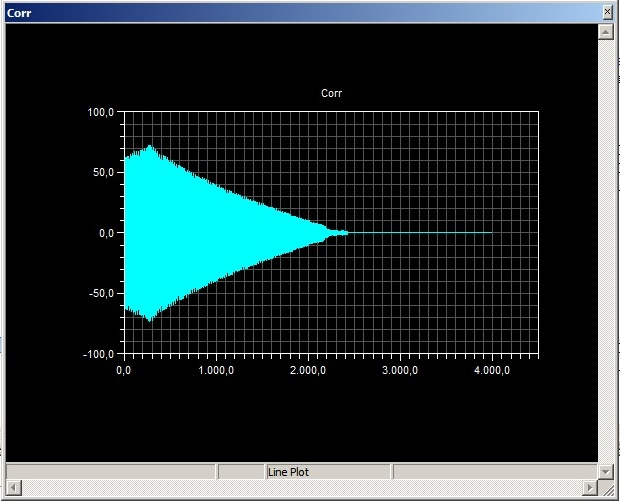
\includegraphics[scale=0.5]{billeder/visualdspplot}
\caption{Plot in VisualDSP++}
\label{fig:visualdspplot}
\end{figure}
\subsection{Memory dump}
A useful feature in VisualDSP++ is Memory dump. We can save the contents of arrays and variables directly onto the computer running VisualDSP++ in ".dat" format. To access this feature go into:
\begin{verbatim}
Memory -> Dump
\end{verbatim}
Set filename, type, size and variable/array name. Matlab can import these files directly.